\section{Related Work}
\label{sec:related}

Descriptor-rich quantum-chemistry datasets divide along two axes: the
chemical envelope they cover and the descriptor families they incorporate.
Smaller, single-purpose releases such as QM9, QMugs, OE62, BDE-db, and
tmQM+ \citep{qm9, qmugs, oe62, bdedb, D5DD00220F} sit below $10^{6}$
structures and typically contain only one descriptor family per dataset.
In contrast, modern force-field training corpora such as ANI-1x/2x, SPICE, GEOM,
transition1x, and OMol25 itself \citep{ani1x, ani2x, spice, geom,
transition1x, levine2026openmolecules2025omol25} routinely
cross $10^{6}$--$10^{8}$ structures but focus only on energies, forces, and
occasionally, a limited set of other features. Even when the latter contain information such as dipoles,
orbital information, and/or partial charges, they typically use only one or two cruder schemes.
OMol-Descriptors-4M encompasses a wider diversity and size vs. existing descriptor datasets, all 
while providing far more descriptors as compared to existing datasets for training MLIPs. 
As this is a broader descriptor dataset, we will only use comparators with a wider 
set of features beyond one partial charge scheme that are also not contained within the 
larger OMol25 dataset. 


\subsection{Comparable-scale descriptor comparators}
\label{sec:related-comparators}

As mentioned, any comparison of descriptors between our dataset and others is moot as existing datasets simply do not cover the diversity
of features within OMol-Descriptors-4M, and typically, do not contain the chemical diversity of OMol25. In lieu of this, we opted to compare
the structural diversity within our dataset to others of comparable descriptor richness, namely, QM7-X, SchNet4AIM, and tmQM+.
QM7-X \citep{qm7x} reaches 4.2M conformers with a rich per-atom data
inventory: Hirshfeld charges, dipoles, atomic $C_{6}$ coefficients,
polarizabilities, van der Waals radii, and a PBE0+MBD energy
decomposition -- but only 6{,}950 unique compositions across CHNOSCl compositions
with at most seven heavy atoms. SchNet4AIM\citep{schnet4aim}, though smaller with only $\sim$3.8K structures, is a closer
analog on the axis of dataset diversity. It contains only CHNO atoms but incorporates QTAIM charges, 
atomic localization indices ($\lambda$), and pairwise
delocalization indices ($\delta$). The tmQM+ dataset \citep{D5DD00220F} is a near precedent on the
descriptor-richness axis for transition-metal chemistry: it incorporates
$\sim$60{,}000 transition-metal complexes with full QTAIM topology
(critical-point scalars, Lagrangian and Hamiltonian kinetic energy
densities, electron localization function, ESP components, gradient and
Laplacian norms, ellipticity, and pairwise QTAIM bond indices) computed
at three levels of theory. 


\begin{table}[h]
\centering
\footnotesize
\setlength{\tabcolsep}{3pt}
\caption{Comparator datasets used for the structural-overlap audit.
``Compositions'' counts unique molecular formulas.}
\label{tab:comparators}
\begin{tabular}{lrrll}
\toprule
Dataset & Structures & Compositions & Chemical Vertical & Descriptors \\
\midrule
QM7-X        & 4.2M  & 6.9k  & CHNOSCl, $\leq 7$ heavy atoms  & Hirshfeld; $C_{6}$, $\alpha$, vdW; PBE0+MBD \\
SchNet4AIM   & 3.9k  & 3.9k  & CHON                         & QTAIM $Q$, $\lambda$, $\delta$ \\
tmQM+~\citep{D5DD00220F}        & 60k   & 60k   &
  \begin{tabular}[t]{@{}l@{}}3d/4d/5d transition-metal \\ complexes \end{tabular} &
  \begin{tabular}[t]{@{}l@{}}Full QTAIM topology, ELF, ESP, \\ kinetic energy densities; 3 LOTs\end{tabular} \\
\midrule
\textbf{Ours} & \textbf{4.0M} & \textbf{1.30M} &
  \begin{tabular}[t]{@{}l@{}}TM, charged, \\ reactive, protein-derived\end{tabular} &
  \begin{tabular}[t]{@{}l@{}}6 charge, 4 bond-order schemes, \\ full QTAIM, fuzzy, ORCA globals\end{tabular} \\
\bottomrule
\end{tabular}
\end{table}

%\subsection{Structural overlap}
%\label{sec:related-overlap}

We confirm that the descriptor breadth above corresponds to genuine
chemistry-space coverage by projecting OMol-Descriptors-4M against the
organic comparators in SOAP-UMAP space (Fig.~\ref{fig:umap_coverage}). The
embedding is fit on a balanced 500-molecule-per-source anchor (1{,}500
points total) using a 6-element common species set
(H, C, N, O, S, Cl). The TM-side overlap with tmQM+ requires a
TM-inclusive SOAP basis and is reported separately in
App.~\ref{app:umap_omol_vs_tmqmplus} where we see that, again, OMol-Descriptors-4M
appears to cover a superset of chemical structures.

\begin{figure}[h]
\centering
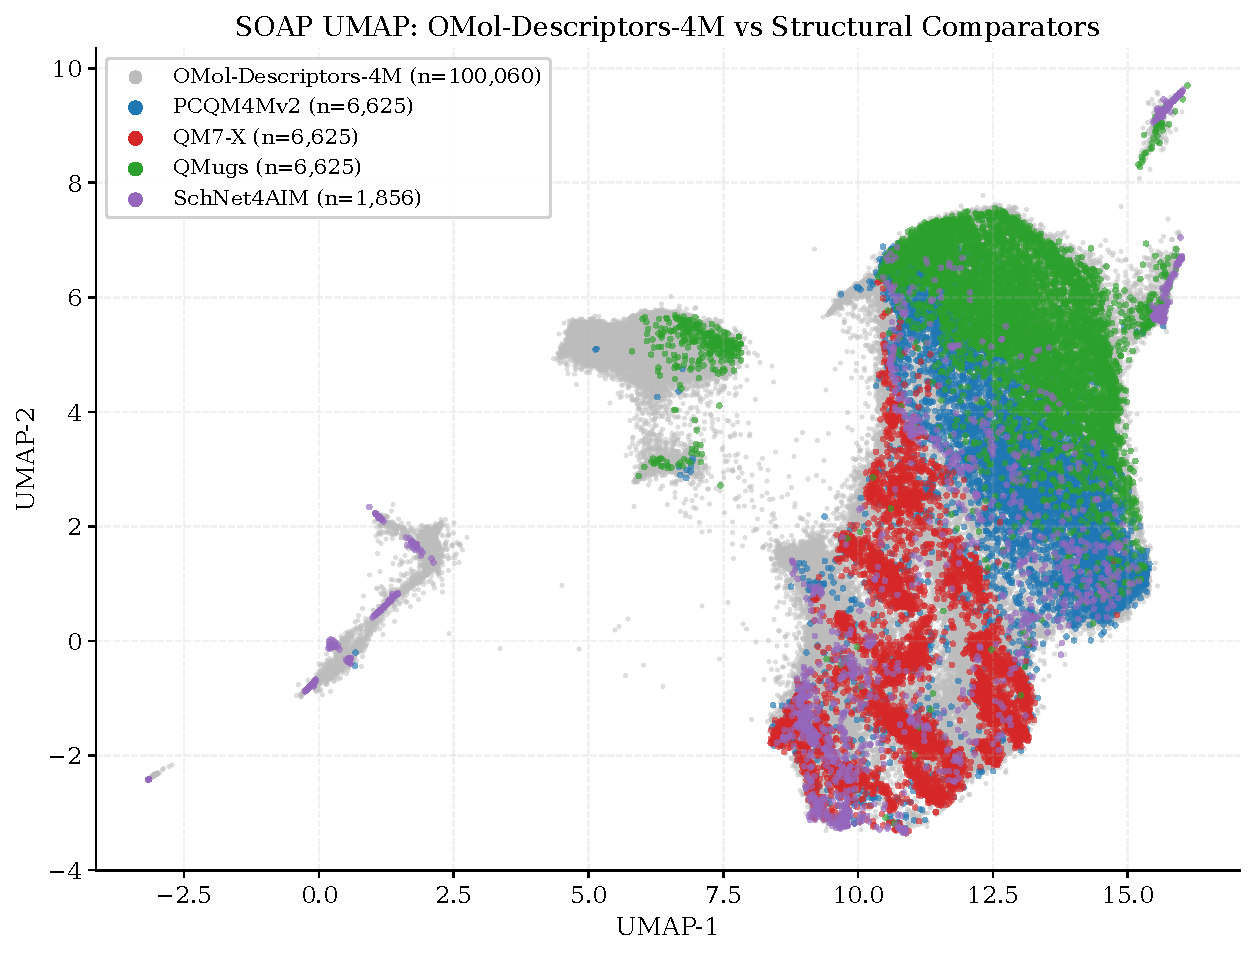
\includegraphics[width=\textwidth]{figures/umap/umap_all_paper.pdf}
\caption{SOAP-UMAP embedding of OMol-Descriptors-4M against the two
organic structural comparator datasets. Each point is a molecule projected via
UMAP fitted on a 500-molecule-per-source balanced subsample. SOAP descriptors use a
6-element species set
(H, C, N, O, S, Cl) common to all three sources.
OMol-Descriptors-4M (gray) is rendered as a background haze to expose
the relative positions of QM7-X and SchNet4AIM.}
\label{fig:umap_coverage}
\end{figure}
